        \documentclass{standalone}
        \usepackage{../BlogTikz}
        \begin{document}

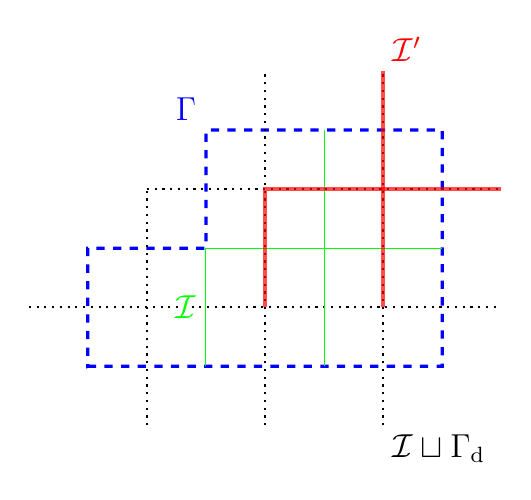
\begin{tikzpicture}[scale=1.5]
\tikzstyle{every node}=[font=\small]
	\draw[very thick, dashed, blue] (-1.5,-0.5) to (1.5,-0.5) to (1.5,1.5) to (-0.5,1.5) to (-0.5,0.5) to (-1.5,0.5) to cycle;
	\node[above left] at (-0.5,1.5) {\large\textcolor{blue}{$\Gamma$}};

	\draw[dotted,thick] (-1,-1) to (-1,1); \draw[dotted,thick] (0,-1) to (0,2); \draw[dotted,thick] (1,-1) to (1,2);
	\draw[dotted,thick] (-2,0) to (2,0); \draw[dotted,thick] (-1,1) to (2,1);
	\node[below right] at (1,-1) {\large$\mathcal{I}\sqcup\Gamma_\mathrm{d}$};

	\draw[green] (-0.5,-0.5) to (-0.5,0.5) to (1.5,0.5);
	\draw[green] (0.5,-0.5) to (0.5,1.5);
	\node[left] at (-0.5,0) {\large\textcolor{green}{$\mathcal{I}$}};

	\draw[red,very thick, opacity=0.7] (0,0) to (0,1) to (2,1);
	\draw[red,very thick, opacity=0.7] (1,0) to (1,2);
	\node[above right] at (1,2) {\large\textcolor{red}{$\mathcal{I}'$}};
\end{tikzpicture}
        \end{document}
